\section{Lecture 5: Tangent Spaces}
Lead question: ``What is the velocity of a curve $\gamma : \mathbb{R} \to M$ at the point $p$ of the curve in $M$?''

\subsection{Velocities}
\begin{definition} Let $(M,\mathcal{O},\mathcal{A})$ be a smooth manifold. Let there be a curve $\gamma : \mathbb{R} \to M$, which is at least $C^1$. Suppose $\gamma(\lambda_0) =p$. The \textbf{velocity} of $\gamma$ at the point $p$ of the curve $\gamma$ is the linear map \\
\begin{equation*}
v_{\gamma, p} : C^{\infty}(M) \linearmapto \mathbb{R} \text{ with }
f \mapsto v_{\gamma,p}(f):= (f \after \gamma)^{\prime}(\lambda_0)
\end{equation*}
where $C^{\infty}(M) := \lbrace f: M \to \mathbb{R} \, | \, f \text{ is a smooth function } \rbrace$ equipped with \\
$(f \oplus g)(p) := f(p) + g(p)$ and $(\lambda \otimes g)(p) := \lambda \cdot g(p)$ is a vector space.
\end{definition}

\textit{Intuition: If the first $\mathbb{R}$ in the picture below is thought of as time, and $f$ as temperature, then $f \after \gamma$ relates time and temperature and $(f \after \gamma)^\prime$ is the rate of change of temperature as you run around the curve.}
\begin{tikzpicture}
  \matrix (m) [matrix of math nodes, row sep=4em, column sep=6em, minimum width=2em]
  {
 \mathbb{R} & M  & \mathbb{R}   \\
};
  \path[->]  
  (m-1-1) edge node [auto] {$\gamma$} (m-1-2)
          edge [bend right=30] node [auto] {$f \after \gamma$} (m-1-3)
  (m-1-2) edge node [auto] {$f $} (m-1-3);
\end{tikzpicture}

\underline{past}: `` $\underbrace{v^i}_{\text{vector in past}} (\partial_i f) = (\underbrace{v^i \partial_i}_{\text{vector as map}})f$ 

\subsection{Tangent vector space}

\begin{definition}
For each point $p \in M$, the \textbf{tangent space} to $M$ at the point $p$ is the set \\
\begin{equation*}
T_p M := \lbrace v_{\gamma, p} \, | \, \text{ for all smooth curves } \gamma \text{ through } p \rbrace
\end{equation*}
\end{definition}

\textbf{Picture}:\\
\begin{tabular}{ p{8cm} | p{8cm} }
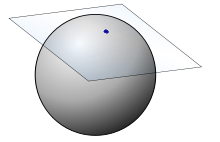
\includegraphics[scale=0.9]{5_Tangent_plane} & 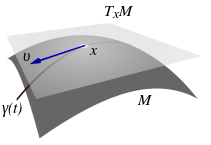
\includegraphics[scale=0.9]{5_Tangential_vector} \\
A pictorial representation of the tangent space $T_xM$ of a single point, x, on a manifold. A vector in this $T_xM$ can represent a possible velocity at x. After moving in that direction to a nearby point, one's velocity would then be given by a vector in the tangent space of that nearby point — a different tangent space, not shown. \textit{By Alexwright at English Wikipedia - Transferred from en.wikipedia to Commons by Ylebru., Public Domain \url{https://commons.wikimedia.org/w/index.php?curid=3941393}} & The tangent space $T_xM$ and a tangent vector $v \in T_xM$, along a curve travelling through $x \in M$. \textit{By derivative work: McSush (talk)Tangentialvektor.png: TNThe original uploader was TN at German Wikipedia - Tangentialvektor.png, Public Domain, \url{https://commons.wikimedia.org/w/index.php?curid=4821938}} \\
\end{tabular}

\textit{\textbf{Caution}: Although the above pictures refer to an ambient space in which $M$ is embedded, the tangent space has been defined intrinsically. There is a velocity corresponding to each curve along a different path in $M$ passing through $p$. Velocity along two different curves could be same, or curves along same paths but having different parameter speeds would yield different velocities.}

\textbf{Observation}: $T_pM$ can be made into a vector space. Define $\oplus$ and $\otimes$ such that

\[
\begin{aligned}
& \begin{aligned}
  \oplus : & T_pM \times T_pM \to Hom(C^\infty(M),\mathbb{R})  \\
  & (v_{\gamma,p} \oplus v_{\delta,p})(\underbrace{f}_{ \in C^{\infty}(M)} ) := v_{\gamma,p}(f) +_{\mathbb{R}} v_{\delta,p}(f) \\
  \end{aligned} \\
& \begin{aligned}
    \odot : & \mathbb{R} \times T_pM \to Hom(C^{\infty}(M),\mathbb{R}) \\
    & (\alpha \odot v_{\gamma,p} )(f) := \alpha \cdot_{\mathbb{R}}  v_{\gamma, p}(f)
\end{aligned}
\end{aligned}
\]
It remains to be shown that 
\begin{enumerate}[i)]
  \item $\exists \, \sigma$ curve : $v_{\gamma,p} \oplus v_{\delta,p} = v_{\sigma,p}$
  \item $\exists \, \tau $ curve : $\alpha \odot v_{\gamma,p} = v_{\tau,p}$
\end{enumerate}
%lazierthanthou: Rest of this notes to be reviewed

\underline{Claim}: $\begin{aligned} & \quad \\ 
  \tau : \mathbb{R} &  \to M  \\
  & \mapsto \tau(\lambda) := \gamma(\alpha  \lambda + \lambda_0) = (\gamma \circ \mu_{\alpha})(\lambda)
\end{aligned}$
where $\begin{aligned} & \quad \\
   \mu_{\alpha}: & \mathbb{R} \to \mathbb{R} \\ 
   & r \mapsto \alpha \cdot r + \lambda_0 \end{aligned}$, 
does the trick.

$\tau(0) = \gamma(\lambda_0) =p$

\[
\begin{aligned}
  v_{\tau,p} & := (f\circ \tau)'(0) = (f\circ \gamma \circ \mu_{\alpha} )'(0) \\ 
  & =  (f\circ \gamma)'(\lambda_0) \cdot \alpha = \\
  & = \alpha \cdot v_{\gamma,p}
\end{aligned}
\]

Now for the sum: %(EY:20151109 ??)
$v_{\gamma,p} \oplus v_{\delta,p} \overset{?}{=} v_{\sigma, p} $
make a \underline{choice} of chart $(\underbrace{U}_{\ni p} , x)$  In cloud: ill definition alarm bells. 

and define:

Claim:
\[
\begin{aligned}
  & \sigma : \mathbb{R} \to M \\
  & \sigma(\lambda) := x^{-1}( \underbrace{ (x\circ \gamma)(\lambda_0 + \lambda)}_{\mathbb{R} \to \mathbb{R}^d}  + (x\circ \delta)(\lambda_1+ \lambda) - (x\circ \gamma)(\lambda_0) )
\end{aligned}
\]
does the trick.
\begin{proof}
Since: 
\[
\begin{aligned}
  \sigma_x(0) & = x^{-1}((x\circ \gamma)(\lambda_0) + (x\circ \delta)(\lambda_1) - (x\circ \gamma)(\lambda_0)) \\
  & = \delta(\lambda_1) = p \end{aligned}
\]
Now:
\[
\begin{aligned}
  v_{\sigma_x,p}(f) & := (f\circ \sigma_x)'(0) =  \\ 
  & = ( \underbrace{ (f\circ x^{-1}) }_{\mathbb{R}^d \to \mathbb{R}}  \circ \underbrace{ (x\circ \sigma_x) }_{\mathbb{R} \to \mathbb{R}^d}  )'(\gamma) = \underbrace{ (x\circ \sigma_x)'(0) }_{(x\circ \gamma)'(\lambda_0) + (x\circ \delta)'(\lambda_1) } \cdot \left( \partial_i (f\circ x^{-1}) \right)(x( \underbrace{ \sigma(0)}_{p} ) ) = \\
  & = (x\circ \gamma)'(\lambda_0)(\partial_i (f\circ x^{-1}) )(x(p)) + (x\circ \delta)(\lambda_1)(\partial_i (f\circ x^{-1})  )(x(p)) \\
  & = (f\circ \gamma)'(\lambda_0) + (f\circ \delta)'(\lambda_1) = \\
  & = v_{\gamma,p}(f) + v_{\delta,p}(f) \quad \, \forall \, f \in C^{\infty}(M)
\end{aligned}
\]

\[
\boxed{ v_{\gamma,p} \oplus v_{\delta,p} = v_{\sigma, p} }
\]
\end{proof}

\begin{tikzpicture}
  \matrix (m) [matrix of math nodes, row sep=4em, column sep=6em, minimum width=2em]
  {
     \mathbb{R} & M  & \mathbb{R}   \\
     & \mathbb{R}^d & \\ 
};
  \path[->]  
  (m-1-1) edge node[auto] {$\sigma$} (m-1-2)
          edge node[sloped, anchor=center, below] {$x \after \sigma$} (m-2-2)
  (m-1-2) edge node[auto] {$x$} (m-2-2)
          edge node[auto] {$f$} (m-1-3)
  (m-2-2) edge node[sloped, anchor=center, below] {$f \after x^{-1}$} (m-1-3);
\end{tikzpicture}


\underline{picture}: (cf. \url{https://youtu.be/pepU_7NJSGM?t=39m5s})

\[
\begin{aligned} 
  \gamma : \mathbb{R} \to M \\
  \delta : \mathbb{R} \to M \end{aligned}
\]
$(\gamma \oplus)(\lambda) := \gamma(\lambda) + \delta(\lambda)$

EY : 20151109 Schuller says adding trajectories is chart dependent, bad. Adding velocities is good.  
\subsection{Components of a vector wrt a chart}

\begin{definition}
  Let $(U,x) \in \mathcal{A}_{\text{smooth}}$.  \\
  Let $\begin{aligned} & \gamma : \mathbb{R} \to U \\ 
    & \gamma(0) = p \end{aligned}$.  

Calculate 
\[
\begin{aligned} 
  v_{\gamma,p}(f) & := (f \after \gamma)'(0) = (\underbrace{ (f\after x^{-1}) }_{\mathbb{R}^d \to \mathbb{R} }  \after \underbrace{ (x\after \gamma)}_{\mathbb{R} \to \mathbb{R}^d}  )'(0) \\
  & = \underbrace{ (x\after \gamma)^{i'}(0) }_{\dot{\gamma}_x^i(0) }  \cdot \underbrace{ (\partial_i(f\after x^{-1} ) )(x(p))  }_{ =: \left( \frac{ \partial f}{ \partial x^i } \right)_p }
\end{aligned}
\]
think cloud $f:M\to \mathbb{R}$
\[
 = \boxed{ \dot{\gamma}_x^i(0) \cdot \left( \frac{ \partial }{ \partial x^i} \right)_p } f \quad \, \forall \, f \in C^{\infty}(M)
\]
$\therefore$ as a map.  

\[
v_{\gamma,p} \underbrace{=}_{\text{use of chart} } \underbrace{ \gamma_x^i(0) }_{ \text{ ``components of the velocity $v_{\gamma,p}$'' } } \underbrace{ \left( \frac{ \partial }{ \partial x^i} \right)}_{ \substack{ \text{ basis elements of the $T_pM$ wrt which the components need to be understood.} \\
\text{ ``chart induced basis of $T_pM$''} } } 
\]
\end{definition}

Picture: \url{https://youtu.be/pepU_7NJSGM?t=1h16s}

\subsection{Chart-induced basis}

\begin{definition}
  $(U,x) \in \mathcal{A}_{\text{smooth}}$ \\
the $\left( \frac{ \partial }{ \partial x^1} \right)_p , \dots , \left( \frac{ \partial }{ \partial x^d} \right)_p \in T_pU \subseteq T_pM$

constitute a \textbf{basis} of $T_pU$

\end{definition}

\begin{proof} remains: linearly independent 
  \[
\begin{gathered}
\lambda^i \left( \frac{ \partial }{ \partial x^i} \right)_p \overset{!}{=} 0  \\
 \Longrightarrow \lambda^i \left( \frac{ \partial }{ \partial x^i} \right)_p(x^j) = \lambda^i \partial_i (\underbrace{ x^j \after x^{-1} }_{} )( x(p)) = \\
 = \lambda^i \delta_i^{\,\,j} = \lambda^j \quad \quad \, j = 1 , \dots , d
\end{gathered} \quad \quad \, \begin{gathered}
  x^j \after x^{-1} : \mathbb{R}^d \to \mathbb{R} \\
  (\alpha^1 , \dots , \alpha^d) \mapsto \alpha^j 
\end{gathered}
\]
in cloud: $x^j : U \to \mathbb{R}$ differentiable




\end{proof}


\begin{corollary}
 $ \text{dim}T_pM = d = \text{dim}M$
\end{corollary}

\underline{Terminology}: $X \in T_pM$ $\to $ $\exists \, \gamma : \mathbb{R} \to M : X = v_{\gamma,p}$ and \\
\phantom{\underline{Terminology}:} $\exists \, \underbrace{ X_1^1 , \dots , X^d }_{\in \mathbb{R} } : X = X^i \left( \frac{ \partial }{ \partial x^i} \right)_p$



\subsection{Change of vector \emph{\underline{components}} under a change of chart}

\ding{56} vector does \textbf{not} change under change of chart.

Let $(U,x)$ and $(V,y)$ be overlapping charts and $p \in U\cap V$.  \\
Let $X \in T_pM$

\[
X^i_{(y)}\cdot \left( \frac{ \partial }{ \partial y^i} \right)_p \underbrace{=}_{(V,y)} X \underbrace{=}_{ (U,x) } X^i_{x} \left( \frac{ \partial }{ \partial x^i} \right)_p
\]
to study change of components formula:
\[
\begin{aligned}
  \left( \frac{ \partial }{ \partial x^i} \right)_p f & = \partial_i(f\after x^{-1} )(x(p)) =  \\
  & = \partial_i (\underbrace{ (f\after y^{-1}) }_{\mathbb{R}^d \to \mathbb{R} } \after (\underbrace{ y\after x^{-1}}_{\mathbb{R}^d \to \mathbb{R}^d} )(x(p)) \\
  & = (\partial_i (y^i\after x^{-1} ) )(x(p)) \cdot (\partial_j (f\after y^{-1}) )(y(p)) = \\
  & = \boxed{ \left( \frac{ \partial y^p}{ \partial x^i} \right)_p \cdot \left( \frac{ \partial f}{ \partial y^j} \right)_p  } f
\end{aligned}
\]
\[
\begin{gathered}
  \Longrightarrow X^i_{(x)} \left( \frac{ \partial y^j}{ \partial x^i} \right)_p \left( \frac{ \partial }{ \partial y^j} \right)_p = X^j_{(y)}\left( \frac{ \partial }{ \partial y^j} \right)_p \\
  \Longrightarrow \boxed{ X^j_{(y)} = \left( \frac{ \partial y^j}{ \partial x^i} \right)_pX^i_{(x)} }
\end{gathered}
\]

\subsection{Cotangent spaces }

$T_pM = V$

trivial $(T_pM)^* := \lbrace \varphi : T_pM \xrightarrow{\sim} \mathbb{R} \rbrace$

\underline{Example}: $f\in C^{\infty}(M)$ 

\[
\begin{aligned}
  (df)_p : & T_p M \xrightarrow{ \sim } \mathbb{R} \\ 
  & X \mapsto (df)_p(X)
\end{aligned}
\]
i.e. $\boxed{ (df)_p \in T_pM^* } $

$(df)_p$ called the gradient of $f$ at the point $p \in M$.  

Calculate components of gradient w.r.t. chart-induced basis $(U,x)$  

\[
\begin{aligned}
  \left( (df)_p \right)_j & := (df)_p\left( \left( \frac{ \partial }{ \partial x^j} \right)_p \right) \\
  & = \left( \frac{ \partial f}{ \partial x^j } \right)_p = \partial_j (f\after x^{-1} )(x(p))
\end{aligned}
\]

\begin{theorem}
  Consider chart $(U,x)  \Longrightarrow x^i : U \to \mathbb{R}$  

\underline{Claim}: $(d x^1)_p, (dx^2)_p, \dots , (dx^d)_p$ basis of $T_p^*M$ 

$\Longrightarrow $ In fact: dual basis: 
\[
(dx^a)_p \left( \left( \frac{ \partial }{ \partial x^b} \right)_p \right) = \left( \frac{ \partial x^a}{ \partial x^b} \right)_p = \dots = \delta_b^a
\]
\end{theorem}

\subsection{Change of \emph{ \underline{components} } of a covector under a change of chart: }

\[
\begin{gathered}
  \underbrace{ T_p^*M }_{ \ni \omega} \text{ with } 
\omega_{(y)} (dy^j)_p =   \omega = \omega_{(x)i} (dx^i)_p  \\
\Longrightarrow \boxed{ \omega_{(y)i} = \frac{ \partial x^j}{ \partial y^i } \omega_{(x)j } }
\end{gathered}
\]
